% Ref: https://www.overleaf.com/latex/templates/emory-poster-template/skpfmpxjnqdh

\documentclass[25pt, a3paper, landscape, margin=10mm, innermargin=15mm, blockverticalspace=15mm, subcolspace=8mm, dvipsnames]{tikzposter} % you need to leave in dvipsnames or else it undoes the orange edge colour??

\usepackage[T1]{fontenc}
\usepackage{helvet}
%\usepackage[utf8]{inputenc}
\usepackage{amsmath}
\usepackage{amsfonts}
\usepackage{amsthm}
\usepackage{amssymb}
\usepackage{mathrsfs}
\usepackage{graphicx}
\usepackage{adjustbox}
\usepackage{enumitem}
\usepackage[backend=bibtex,style=numeric, citestyle=ieee]{biblatex}
\usepackage{xpatch}
\usepackage{xcolor}
\usepackage{multicol}
\usepackage{lipsum}

\setlength{\columnsep}{2.5cm}
%\setlength{\columnseprule}{1mm}
\pagecolor{Dandelion}

% Ref: https://latex-cookbook.net/poster/
\renewcommand*{\familydefault}{\sfdefault}% Let's have a sans serif font

% set theme parameters
\tikzposterlatexaffectionproofoff
\usepackage{anyfontsize}
\usetheme{Default}
\usebackgroundstyle{Default}
\definecolor{epccnavy}{HTML}{1D2A3D}
\definecolor{universityred}{HTML}{D50032}
\colorlet{backgroundcolor}{white} % <<< this makes bg white
\colorlet{framecolor}{epccnavy}%Dandelion}
\colorlet{titlefgcolor}{epccnavy}
\colorlet{blocktitlebgcolor}{epccnavy}
\colorlet{blocktitlefgcolor}{white}
\colorlet{blockframecolor}{epccnavy}

% \definetitlestyle{sampletitle}{
%     width=800mm, 
%     roundedcorners=20, 
%     linewidth=10pt, 
%     innersep=10pt,
%     titletotopverticalspace=15mm, titletoblockverticalspace=25mm 
% }{
% \begin{scope}[line width=\titlelinewidth, rounded corners=\titleroundedcorners]
% \draw[color=blocktitlebgcolor, fill=titlebgcolor]
% (\titleposleft,\titleposbottom) rectangle (\titleposright,\titlepostop);
% \end{scope}
% }
% \usetitlestyle[]{sampletitle}


% Ref: https://tex.stackexchange.com/questions/309713/modify-font-style-in-title-of-tikzposter
\settitle{ \centering
\vbox{
    %\@titlegraphic \\[\TP@titlegraphictotitledistance] \centering
    \color{titlefgcolor} {\sffamily \bfseries \huge  \textsc{\@title} \par}
    \color{universityred} {\sffamily \bfseries \huge \subtitle}   
    \vspace*{0.5em}
    \begin{flushleft}
    {\color{titlefgcolor} {\sffamily \huge \@author}
    \hspace{1em}
    {\sffamily \LARGE \@institute \par}}
    \end{flushleft}
}
}
\makeatother

% Ref: https://tex.stackexchange.com/questions/180234/how-can-i-make-my-title-wrap-in-a-tikzposter
\makeatletter
\def\title#1{\gdef\@title{\scalebox{\TP@titletextscale}{%
			\begin{minipage}[t]{\linewidth}
				%\centering
				#1
			\par
				\vspace{0.5em}
			\end{minipage}%
}}}
\makeatother

% Ref: https://tex.stackexchange.com/questions/263563/add-logos-beyond-the-title-tikzposter
%\title{\parbox{\linewidth}{Do Research Software Developer Personas Exist? Are *YOU* an RS-10X? \\ Identifying Distinct Developer/Repository Interaction Types by Mining GitHub Data}}
\title{\parbox{\linewidth}{Do Research Software Developer Personas Exist? Are *YOU* an RS-10X?}}
\newcommand{\subtitle}{Identifying Distinct Developer/Repository Interaction Types by Mining GitHub Data}
\author{\textbf{Felicity `Flic' Anderson\textsuperscript{$\dagger$}}, Julien Sindt\textsuperscript{$\dagger$} and Neil Chue Hong\textsuperscript{$\dagger$}}
\institute{\textsuperscript{$\dagger$}EPCC, University of Edinburgh}
%\titlegraphic{
\includegraphics{epcclogo.png}}

\makeatletter
\newcommand\insertlogoi[2][]{\def\@insertlogoi{\includegraphics[#1]{#2}}}
%\newcommand\insertlogoi[2][]{\def\@insertlogoi{\hspace*{0.5in}\includegraphics[#1]{#2}}}
\newcommand\insertlogoii[2][]{\def\@insertlogoii{\includegraphics[#1]{#2}}}
%\newcommand\insertlogoii[2][]{\def\@insertlogoii{\hspace*{-7.5in}\includegraphics[#1]{#2}}}
%\newcommand\insertlogoiii[2][]{\def\@insertlogoiii{\includegraphics[#1]{#2}}}
\newlength\LogoSep
\setlength\LogoSep{0pt}

\insertlogoi[width=14cm]{informaticsUoE.png}
\insertlogoii[width=15cm]{epcclogo.png}
%\insertlogoii[width=15cm]{EpccANDEmailQRsidebyside.png}

\renewcommand\maketitle[1][width=800mm]{  % #1 keys
	\normalsize
	\setkeys{title}{#1}
	% Title dummy to get title height
	\node[transparent,inner sep=\TP@titleinnersep, line width=\TP@titlelinewidth, anchor=north, minimum width=\TP@visibletextwidth-2\TP@titleinnersep]
	(TP@title) at ($(0, 0.5\textheight-\TP@titletotopverticalspace)$) {\parbox{\TP@titlewidth-2\TP@titleinnersep}{\TP@maketitle}};
	\draw let \p1 = ($(TP@title.north)-(TP@title.south)$) in node {
		\setlength{\TP@titleheight}{\y1}
		\setlength{\titleheight}{\y1}
		\global\TP@titleheight=\TP@titleheight
		\global\titleheight=\titleheight
	};
	
	% Compute title position
	\setlength{\titleposleft}{-0.5\titlewidth}
	\setlength{\titleposright}{\titleposleft+\titlewidth}
	\setlength{\titlepostop}{0.5\textheight-\TP@titletotopverticalspace}
	\setlength{\titleposbottom}{\titlepostop-\titleheight}
	
	% Title style (background)
	\TP@titlestyle
	
	% Title node
	\node[inner sep=\TP@titleinnersep, line width=\TP@titlelinewidth, anchor=north, minimum width=\TP@visibletextwidth-2\TP@titleinnersep]
	at (0,0.5\textheight-\TP@titletotopverticalspace)
	(title)
	{\parbox{\TP@titlewidth-2\TP@titleinnersep}{\TP@maketitle}};
	
	\node[inner sep=0pt,anchor=west] 
	at ([xshift=-\LogoSep]title.west)
	{\@insertlogoi};
	
	\node[inner sep=0pt,anchor=east] 
	at ([xshift=\LogoSep]title.east)
	{\@insertlogoii};
	
	% Settings for blocks
	\normalsize
	\setlength{\TP@blocktop}{\titleposbottom-\TP@titletoblockverticalspace}
}
\makeatother

% begin document
\begin{document}
%\useblockstyle{Basic}
\maketitle

\begin{columns}\column{.45}

\block{0: Research Context}{
    \vspace{1em}
    {\fontsize{60}{60}\selectfont 
    %\vspace{1em}
    \begin{itemize}
        \item What is \textbf{Research Software}? Why is it often so bad?
        \vspace{1em}
        \item What are development practices in 'typical' real world RS projects?
        \vspace{1em}
        \item Are there differing `clusters' of practices?
        \vspace{1em}
        \item Can we identify those clusters as  RS Personas?
    \end{itemize}
    \vspace{1em}
    }
    {\fontsize{70}{70}\selectfont
    \textbf{Use assignment and contributions data to look for RS 'superstar' developers...}  
    %\vspace{1em}
    }        % via https://tex.stackexchange.com/a/499070
} 
\block{1: Research Goals \& Methods}{
\begin{multicols}{2}
    {\fontsize{60}{60}\selectfont 
        Mining \textbf{GitHub} repository data
        \vspace{1em}

        Focusing on Issue Tickets / Pull Requests in 10 largeish repos 
        \vspace{1em}

        Assignment \thickapprox  \textit{'responsibility'}  

        Commits \thickapprox \textit{'activity'} 
        
        \begin{tikzfigure}[]
            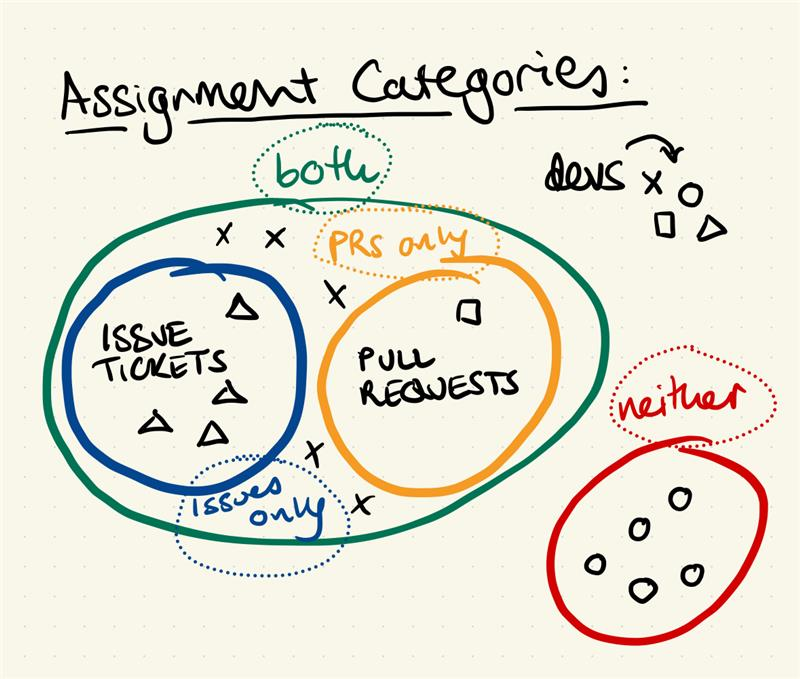
\includegraphics[width=0.85\linewidth]{AssignmentCategories.jpg}
        \end{tikzfigure}
} 
\end{multicols}
}

\column{.55}
\block{2: (Some) Results}{
        \begin{tikzfigure}[]
        %\setlength{\belowcaptionskip}{-8pt}
            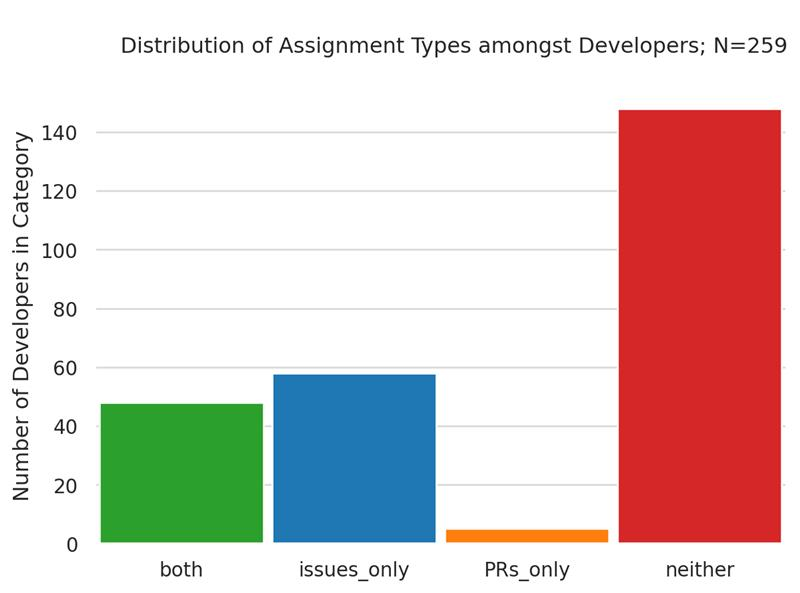
\includegraphics[width=0.55\linewidth]{DistributionOfAssignmentTypes.jpg}
        \end{tikzfigure}
    {\fontsize{60}{60}\selectfont 
    Only $\sim$20\% of devs assigned to BOTH tickets \& PRs... 

    \begin{tikzfigure}[]
        %\setlength{\belowcaptionskip}{-8pt}
        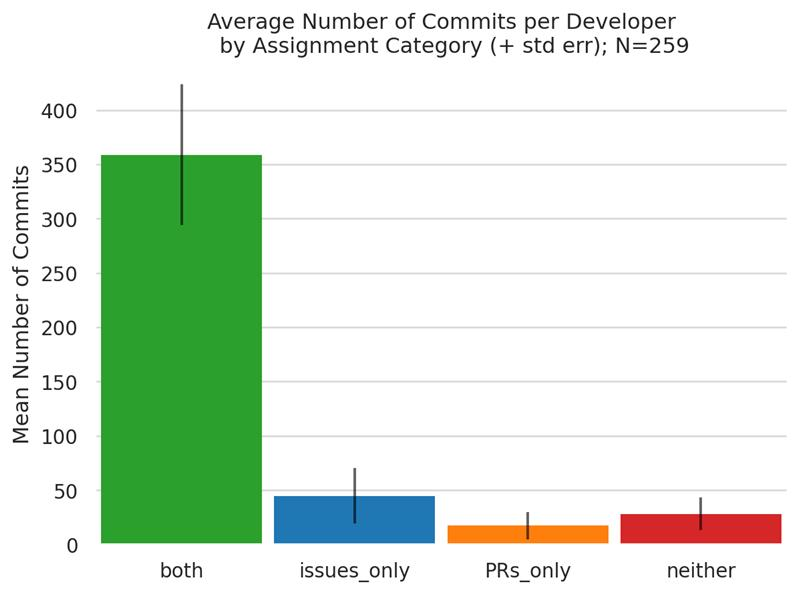
\includegraphics[width=0.55\linewidth]{AverageCommitsByCategory.jpg}
    \end{tikzfigure}
    
    ... But their commit numbers are higher... 
    
    \vspace{1em}
    \textbf{Find out more at my poster!}
    }
}
\end{columns}
\end{document}